% !TEX root = ../presentation.tex

\subsection[Matrix Fisher]{Attitude Uncertainty using Matrix Fisher}


\begin{frame}
\frametitle{Matrix Fisher Distribution on $\SO$}
\begin{itemize}
\item Matrix Fisher Distribution: $\mathcal{M}(F)$
	\begin{itemize}
	\item Probability density defined by a \Emph{matrix parameter} $F\in\Re^{3\times 3}$
\only<1>{

	    \centerline{
	    \begin{beamercolorbox}[wd=10cm,sep=0.0cm,center,rounded=true,shadow=true]{numerical}
		$\displaystyle R\sim\mathcal{M}(F)\quad\Leftrightarrow\quad p(R) \propto  \exp(\mathrm{tr}[F^T R])$
		\end{beamercolorbox}}
		}
\only<2->{

	    \centerline{
	    \begin{beamercolorbox}[wd=10cm,sep=0.0cm,center,rounded=true,shadow=true]{numerical}
                {\small$\displaystyle p(R) = \frac{1}{c(F)}  \exp(\mathrm{tr}[F^T R])$}
		\end{beamercolorbox}}
}
\pause
	\item Normalizing constant $c(F)$ introduced for $\int_{\SO} p(R) dR =1$
%	\item Haar measure $dR$ scaled such that $\int_{\SO} dR =1$
	\item Comparable to a \Emph{Gaussian distribution on $\Re^3$} defined by 9 parameters
	\end{itemize}
\pause
\only<1-3>{\item Singular Value Decomposition of $F$

	\centerline{
	\begin{beamercolorbox}[wd=\textwidth,sep=0.0cm,center,rounded=true,shadow=true]{numerical}
	\vspace*{-0.5cm}
	\begin{align*}
	F & = U' S' (V')^T\\
	&= \begin{bmatrix} & & \\ u'_1 & u'_2 & u'_3 \\ & & \end{bmatrix}
	\begin{bmatrix} s'_1 & 0 & 0\\ 0 & s'_2 & 0 \\ 0 & 0 & s'_3 \end{bmatrix}
	\begin{bmatrix} & (v_1')^T & \\ & (v_2')^T & \\ & (v_3')^T & \end{bmatrix}
	\end{align*}\vspace*{-0.3cm}
	\end{beamercolorbox}}

	\begin{itemize}
	\item Positive singular values: $s_1'\geq s_2'\geq s_3'\geq 0$
	\item $U',V'\in\Re^{3\times 3}$ are orthogonal, but not neccessarily in $\SO$ . 
	\end{itemize}}
\only<4>{\item \Emph{\textit{Proper}} Singular Value Decomposition of $F$

	\centerline{
	\begin{beamercolorbox}[wd=\textwidth,sep=0.0cm,center,rounded=true,shadow=true]{numerical}
	\vspace*{-0.5cm}
	\begin{align*}
	F & = U S V^T\\
	&= \begin{bmatrix} & & \\ u'_1 & u'_2 & \Emph{\mathrm{det}[U']}u'_3 \\ & & \end{bmatrix}
	\begin{bmatrix} s'_1 & 0 & 0\\ 0 & s'_2 & 0 \\ 0 & 0 & \Emph{\mathrm{det}[U'V']}s'_3 \end{bmatrix}
	\begin{bmatrix} & (v_1')^T & \\ & (v_2')^T & \\ & \Emph{\mathrm{det}[V']}(v_3')^T & \end{bmatrix}
	\end{align*}\vspace*{-0.3cm}
	\end{beamercolorbox}}
	
	\begin{itemize}
	\item $s_1\geq s_2\geq |s_3|\geq 0$,\quad $s_1+s_2\geq s_1+s_3\geq s_2+s_3\geq 0$
	\item $U,V\in\SO$
	\end{itemize}}
		
\end{itemize}
\end{frame}
<`0`>
\begin{frame}
\frametitle{Matrix Fisher Distribution on $\SO$}
\begin{itemize}
\item Shape of Matrix Fisher Distribution with $F=USV^T$
	\begin{itemize}
	\item \Emph{Mean attitude} : $UV^T$
	\item \Emph{Principal axes} : columns of $U$
	\item \Emph{Dispersion} along the $i$-th principal axis: $s_j+s_k$
	\end{itemize}
\vspace*{0.3cm}\pause
\end{itemize}
\vspace*{-0.3cm}
\begin{columns}[t]
\begin{column}{0.32\textwidth}
\only<1>{
\begin{tikzpicture}
\node[opacity=0.3,outer sep=0pt,inner sep=0pt] at (0,0) {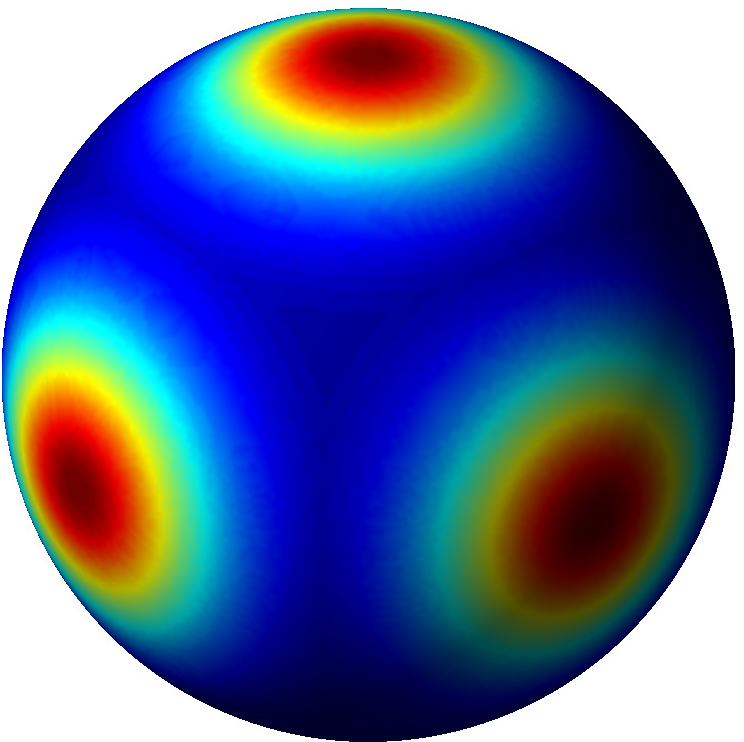
\includegraphics[height=0.4\textheight,width=1\columnwidth, keepaspectratio]{figures/2017AAS_matrix_fisher/TAC16_vis_1}};
\end{tikzpicture}
\centerline{\footnotesize $F_1=5I_{3\times 3}$}
\centerline{\footnotesize $U_1V_1^T=I_{3\times 3},\, U_1=I_{3\times 3}$}
\centerline{\footnotesize $S_1=\mathrm{diag}[5,5,5]$}
}
\only<2->{
\begin{tikzpicture}
\node[opacity=1,outer sep=0pt,inner sep=0pt] at (0,0) {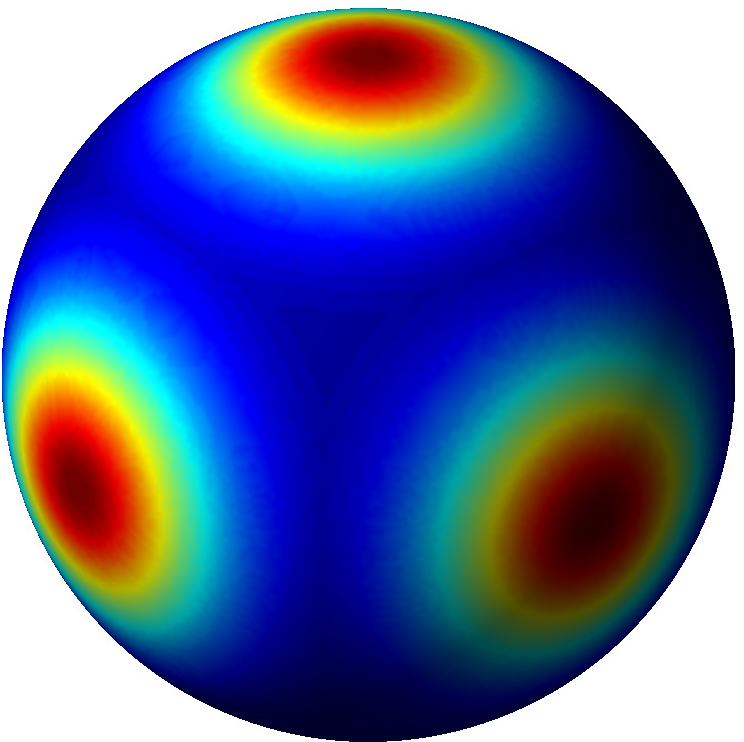
\includegraphics[width=1\columnwidth,height=0.4\textheight, keepaspectratio]{figures/2017AAS_matrix_fisher/TAC16_vis_1}};
\end{tikzpicture}
\centerline{\footnotesize $F_1=5I_{3\times 3}$}
\centerline{\footnotesize $U_1V_1^T=I_{3\times 3},\, U_1=I_{3\times 3}$}
\centerline{\footnotesize $S_1=\mathrm{diag}[5,5,5]$}
}
\end{column}
\pause
\begin{column}{0.32\textwidth}
\only<1,2>{
\begin{tikzpicture}
\node[opacity=0.3,outer sep=0pt,inner sep=0pt] at (0,0) {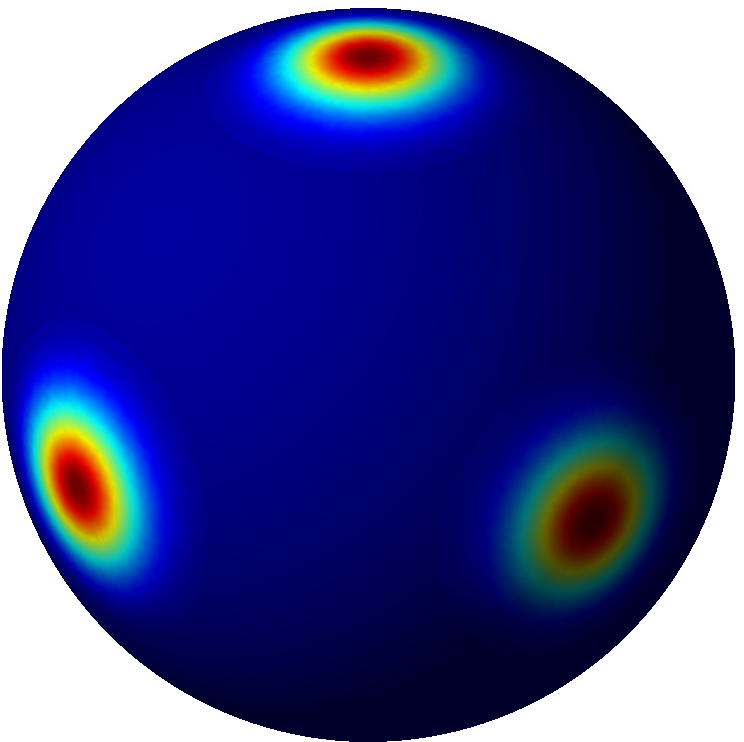
\includegraphics[width=1\columnwidth,height=0.4\textheight,keepaspectratio]{figures/2017AAS_matrix_fisher/TAC16_vis_2}};
\end{tikzpicture}
}
\only<3->{
\begin{tikzpicture}
\node[opacity=1,outer sep=0pt,inner sep=0pt] at (0,0) {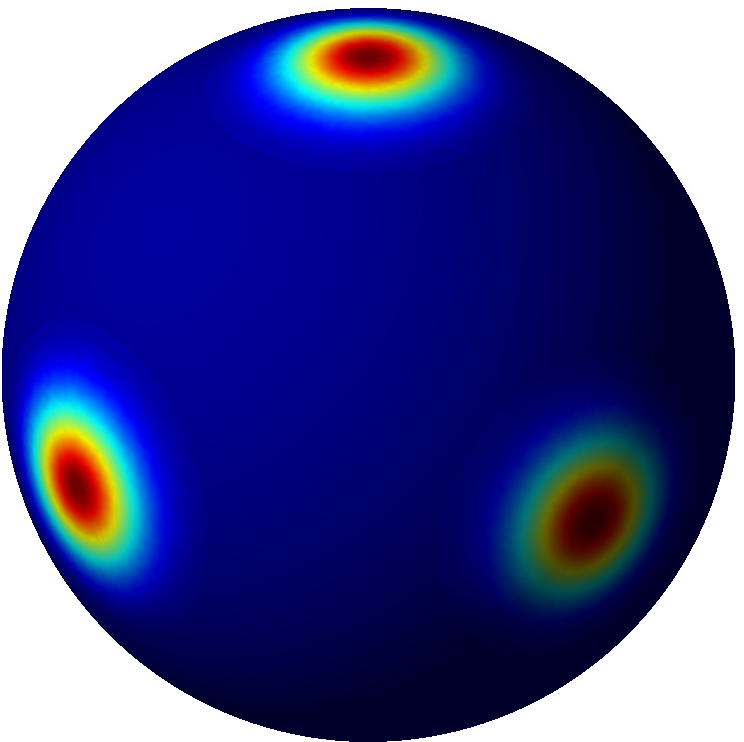
\includegraphics[width=1\columnwidth,height=0.4\textheight,keepaspectratio]{figures/2017AAS_matrix_fisher/TAC16_vis_2}};
\end{tikzpicture}
}
\centerline{\footnotesize $F_2=20I_{3\times 3}$}
\centerline{\footnotesize $U_2V_2^T=I_{3\times 3},\, U_2=I_{3\times 3}$}
\centerline{\footnotesize $S_2=\mathrm{diag}[20,20,20]$}
\end{column}
\pause
\begin{column}{0.32\textwidth}
\only<1,2,3>{
\begin{tikzpicture}
\node[opacity=0.3,outer sep=0pt,inner sep=0pt] at (0,0) {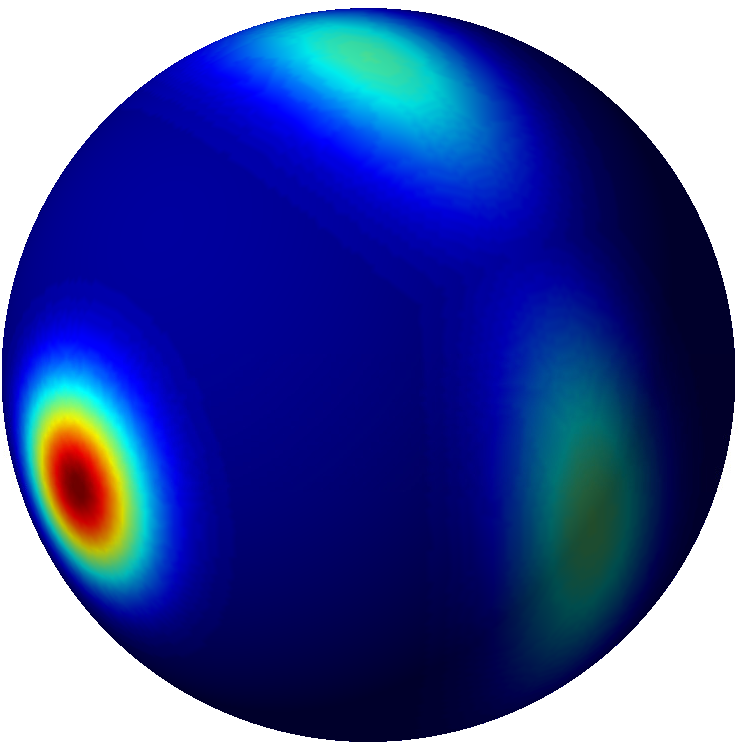
\includegraphics[width=1\columnwidth,height=0.4\textheight,keepaspectratio]{figures/2017AAS_matrix_fisher/TAC16_vis_3}};
\end{tikzpicture}
}
\only<4->{\hspace*{-0.0cm}
\begin{tikzpicture}
\node[opacity=1,outer sep=0pt,inner sep=0pt] at (0,0) {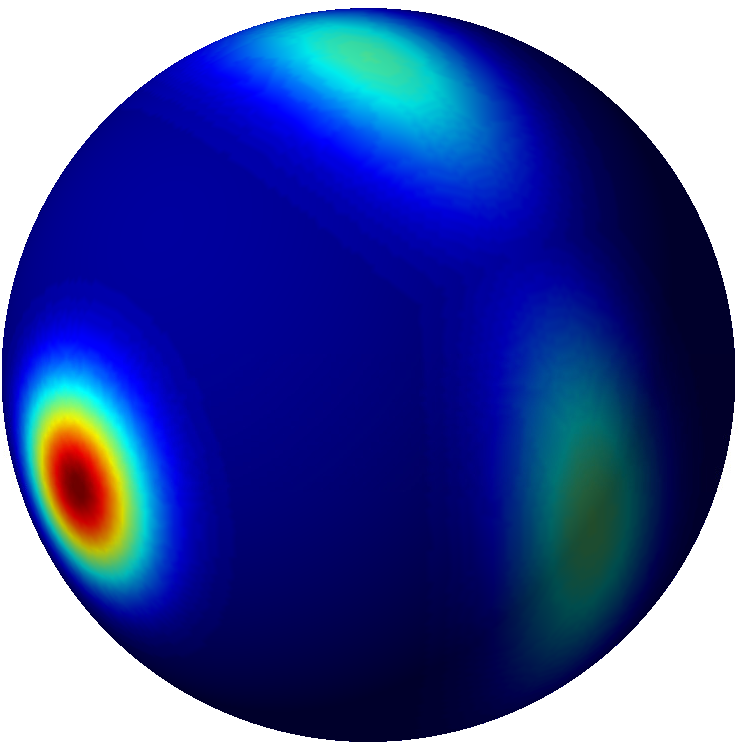
\includegraphics[width=1\columnwidth,height=0.4\textheight,keepaspectratio]{figures/2017AAS_matrix_fisher/TAC16_vis_3}};
% \draw[arrows={-Triangle[angle=30:4pt]}] (-2.1,-1.8) -- (-2.1,-1.2);
% \draw[arrows={-Triangle[angle=30:4pt]}] (-2.1,-1.8) -- (-2.5,-2.0);
% \draw[arrows={-Triangle[angle=30:4pt]}] (-2.1,-1.8) -- (-1.7,-2.0);
% \node at (-2.4,-2.15) {\scriptsize $e_1$};
% \node at (-1.7,-2.15) {\scriptsize $e_2$};
% \node at (-1.9,-1.4) {\scriptsize $e_3$};
\end{tikzpicture}
}
\centerline{\footnotesize $F_3=\mathrm{diag}[25,5,1]$}
\centerline{\footnotesize $U_3V_3^T=I_{3\times 3},\, U_3=I_{3\times 3}$}
\centerline{\footnotesize $S_3=\mathrm{diag}[25,5,1]$}
\end{column}
\end{columns}
\end{frame}

\begin{frame}
\frametitle{Attitude Estimation}

\begin{itemize}
\item \Emph{Attitude Estimation} Problem Formulation
	\begin{itemize}
	\item Consider a \Emph{stochastic differential equation}
	\[ (R^T dR)^\vee = \Omega dt + H dW,\]
	with a measured angular velocity $\Omega\in\Re^3$, a scaled Wiener process $HdW$ representing measurement noise
	\item Initial attitude follows a \Emph{matrix Fisher distribution}: $R(0)\sim\mathcal{M}(F(0))$
	\item Attitude is measured repeatedly
	\item \Emph{Goal}: determine the current distribution of the attitude uncertainty
	\end{itemize}
\vspace*{0.3cm}\pause
\item \Emph{Bayesian Estimation} with Matrix Fisher Distribution on $\SO$
	\begin{itemize}
	\item \Emph{Assumed density filter}: estimation constructed by $R(t)\sim\mathcal{M}(F(t))$
	\item \Emph{Propagation}
		\begin{itemize}
		\item First-order Propagation
		\item Unscented Transform
		\end{itemize}
	\item \Emph{Measurement Update}
	\end{itemize}
\end{itemize}
\end{frame}
